\section{Results: Four Routes, One Outcome}
\label{sec:results}

\subsection{The frontier}

Fig.~\ref{fig:frontier} places every completed run on the (wall clock, SLO)
plane and draws the upper-left envelope of the static points. Table~\ref{tab:runs}
gives the numbers and each controller's signed distance from that envelope.

The result is unambiguous. Of nine controller variants, none is above the
envelope. The best, a growth-reserve setting of one round instead of the
default three, lands $+0.20$ percentage points above the line---inside the
run-to-run spread of the same configuration, which we measured at
2.2--4.1\%---and we therefore record it as \emph{on} the line rather than
above it.

Two features of the front are worth noting before the negative results.
The envelope is steep between 213 and 236 minutes (0.76\,pp per minute) and
shallow thereafter (0.18\,pp per minute), so the cost of buying SLO by
retreating from the fast end is high. And $W$ is not monotone in concurrency:
five sessions (260.9\,min) is \emph{slower} than four (213.0\,min), because
the per-step cost rises faster than the request count does. We return to this
non-monotonicity in \S\ref{sec:model}, where it turns out to be the first
appearance of the mechanism that drives the whole frontier.

\begin{table}[tb]
  \caption{All completed runs. $\Delta$ is the signed distance from the
  static envelope at that wall clock; positive would mean a genuine win.
  Three controller runs stopped 1--4 steps short of 999 (\texttt{hz0} 995,
  \texttt{hz2} 997, \texttt{rg4} 998); they are listed with their measured
  values and not treated as full runs.}
  \label{tab:runs}
  \centering
  \small
  \begin{tabular}{lrrrr}
    \toprule
    Policy & Wall (min) & Conc. & SLO (\%) & $\Delta$ (pp) \\
    \midrule
    \multicolumn{5}{l}{\emph{Static caps}}\\
    cap1              & 527.4 & 1.00 & 94.8 & --- \\
    cap2              & 304.2 & 1.99 & 89.5 & $-$2.2 \\
    cap3 (fixed)      & 258.7 & 2.89 & 74.4 & $-$10.7 \\
    cap4              & 249.9 & 3.94 & 55.7 & $-$27.9 \\
    cap5              & 260.9 & 4.89 & 27.1 & $-$58.4 \\
    \midrule
    \multicolumn{5}{l}{\emph{Static caps + HiCache}}\\
    cap2+HC           & 295.0 & 1.99 & 91.6 & \emph{anchor} \\
    cap3+HC           & 236.4 & 2.93 & 81.1 & \emph{anchor} \\
    cap4+HC           & 213.0 & 3.93 & 63.4 & \emph{anchor} \\
    \midrule
    \multicolumn{5}{l}{\emph{\sys{} controller variants}}\\
    horizon$=$1       & 255.8 & 2.58 & 84.8 & $+$0.20 \\
    horizon$=$3 (base)& 291.3 & 2.06 & 89.8 & $-$1.14 \\
    horizon$=$2       & 306.1 & 2.22 & 86.9 & $-$4.85 \\
    resident base     & 295.5 & 2.40 & 83.8 & $-$7.82 \\
    horizon$=$0       & 290.0 & 2.69 & 77.2 & $-$13.5 \\
    horizon$=$1, hw off & 310.9 & 2.77 & 72.3 & $-$19.6 \\
    no gate, no resv. & 272.3 & 3.25 & 66.6 & $-$20.9 \\
    running gate$=$4  & 282.3 & 3.03 & 64.3 & $-$24.0 \\
    all throttles off & 415.0 & 2.58 & 46.1 & $-$48.7 \\
    \bottomrule
  \end{tabular}
\end{table}

\subsection{Route 1: the accounting base}

Our controller's projection (Eq.~\ref{eq:proj}) charges a session for its full
context even while it is parked in a tool wait, when its KV is evictable and
therefore absent from the engine's reported occupancy. We argued this was a
double charge and removed it, admitting on engine telemetry alone.

The charge is not double. Removing it did admit more---engine occupancy rose
from 41.0\% to 52.2\% of the pool---and the round-1+ prefix hit rate held at
80.8\% against 80.6\%, so no eviction spiral occurred. But the run was
4.2 minutes \emph{slower} and lost 6.0\,pp of SLO. Per \S\ref{sec:model}, the
extra occupancy raised both $\overline{R}$ and $\tau$ (31.3\,ms against
23.8\,ms), and the two cancelled.

We note that this claim had already been falsified once by source inspection:
SGLang's \texttt{token\_usage} subtracts evictable blocks, so a parked
session's prefix is genuinely not counted, and charging for it reserves
capacity that really will be needed back. The end-to-end measurement agrees
with the source reading.

\subsection{Route 2: the growth reserve}

Sessions grow by roughly 2.5K tokens per round, so the controller reserves
capacity for the next \texttt{horizon} rounds. We swept the horizon over
$\{0,1,2,3\}$ and the reserve is not a free parameter to be minimised:
Fig.~\ref{fig:horizon} shows the response is non-monotone. Removing the
reserve entirely costs 13.5\,pp of SLO, and a reserve of two rounds is
15 minutes \emph{slower} than three. The optimum is at one round, and there it
touches the static front and stops.

\subsection{Route 3: the hard ceiling}

Lowering the budget fraction is the crudest available knob and behaves as the
other routes do: it slides the operating point along the front. We report it
only for completeness, since it adds no mechanism.

\subsection{Route 4: execution granularity}
\label{sec:results:gate}

The first three routes all assume that what a controller can set is \emph{how
many sessions are resident}. A static cap sets the same quantity, so it is
unsurprising that they land in the same place. The fourth route attacks the
assumption instead: because a large fraction of live sessions are parked at
any instant, a cap on \emph{resident} sessions leaves the engine idle whenever
all residents happen to be parked. Capping the \emph{running-request} count
instead should keep the engine busy while leaving the resident count high.

The permit design supports this directly: a paused session finishes its
current round and blocks before its next one, and resumes when the controller
re-admits it. We implemented it as a gate on the engine's own
\texttt{num\_running\_reqs} and swept the gate over $\{2,4\}$.

It does not work, and the reason is structural rather than a tuning matter.
Since a live session is running about 45\% of the time, the running count is
approximately $0.45 \times (\text{live count})$. Constraining the live count to
$N$ therefore constrains the running count to $0.45N$, which is below the
gate---so the gate can only throttle, never pin. Both repairs fail: without a
constraint on admission, a paused session is re-admitted on the next cycle and
blocks for at most one 2\,s cycle; with one, the policy is a session cap again.
The obstacle is granularity---\texttt{paused} takes effect at round
boundaries, while pinning an instantaneous count requires control the
permit mechanism does not have.

The measured outcome matches: the gate drove running concurrency from 1.42 to
1.29 and live sessions from 2.78 to 1.91. It tightened rather than pinned, and
a tightening is another cap.

\begin{figure}[tb]
  \centering
  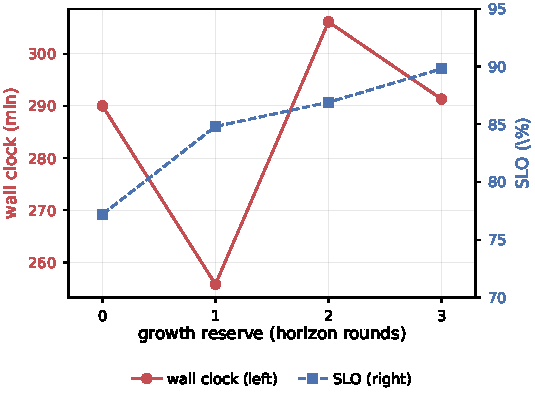
\includegraphics[width=\columnwidth]{figs/fig6_horizon.pdf}
  \caption{The growth reserve is not a free parameter. Removing it costs
  13.5\,pp of SLO; two rounds is 15 minutes slower than three. The optimum at
  one round touches the static front and does not cross it.}
  \label{fig:horizon}
\end{figure}
